\documentclass[10pt,a4paper]{article}
\usepackage[margin=1in]{geometry}
\usepackage{amsmath,amsfonts,amssymb,tikz}
\usepackage{longtable}

\usepackage{hyperref}
\usepackage{graphicx}
\title{Machine Learning Exam Cheat Sheet}
\author{}
\date{}
\begin{document}
\maketitle

\section*{Key Concepts}
\section*{Biases in Machine Learning}

\subsection*{Inductive Bias}
Inductive bias refers to the assumptions a learning algorithm makes to generalize beyond the training data. It enables the algorithm to choose among multiple hypotheses consistent with the data, making learning possible. For instance, decision tree algorithms assume simpler trees are more likely correct, adhering to Occam's Razor. While necessary, the strength of inductive bias determines the trade-off between flexibility and overfitting. A weak inductive bias allows exploration of diverse hypotheses but risks overfitting, whereas a strong bias ensures efficiency at the cost of flexibility.

\subsection*{Hypothesis Space Bias}
Hypothesis space bias arises from the set of hypotheses the algorithm considers. By limiting the hypothesis space, the algorithm becomes computationally efficient but may exclude the true target function. For example, linear regression restricts solutions to linear relationships, which might not capture nonlinear patterns. This bias ensures tractability but requires the hypothesis space to align closely with the true concept. Careful design of the hypothesis space is critical to balancing computational constraints and accuracy.

\subsection*{Search Bias}
Search bias refers to how an algorithm explores the hypothesis space during learning. Algorithms like ID3 use greedy search strategies, prioritizing locally optimal splits based on metrics like information gain. While efficient, this approach may lead to suboptimal solutions by missing global optima. Search bias influences the speed of learning and the type of solutions reached. It complements hypothesis space bias by determining the exploration method within the given constraints.

\subsection*{Representation Bias}
Representation bias stems from how data and hypotheses are structured. The choice of representation affects what patterns the algorithm can learn. For example, representing data in binary format allows Boolean logic-based algorithms to perform efficiently but limits their ability to capture complex patterns. This bias is inherently linked to the domain knowledge used to preprocess data and design the learning task. A well-chosen representation enhances learning, while a poor one hinders it.

\subsection*{Model Selection Bias}
Model selection bias concerns the trade-off between high- and low-bias models. Simpler models (high bias) generalize better but may underfit, while complex models (low bias) capture more details but risk overfitting. For example, linear regression is a high-bias approach compared to polynomial regression, which offers lower bias and higher variance. Selecting the appropriate model depends on the problem complexity and the available data.


\subsection*{Bias-Variance Trade-off}
\begin{itemize}
    \item \textbf{Bias}: Error from overly simplistic assumptions.
    \item \textbf{Variance}: Error from sensitivity to fluctuations in the training set.
    \item \textbf{Trade-off}: Aim for low total error:
    \[
    \text{Total Error} = \text{Bias}^2 + \text{Variance} + \text{Irreducible Error}.
    \]
\end{itemize}
\begin{longtable}{|p{3cm}|p{5cm}|p{5cm}|p{3cm}|}
\hline
\textbf{Model} & \textbf{Core Characteristics} & \textbf{Strengths} & \textbf{Limitations} \\
\hline
\endfirsthead
\hline
\textbf{Model} & \textbf{Core Characteristics} & \textbf{Strengths} & \textbf{Limitations} \\
\hline
\endhead
\hline
\endfoot
\hline
\endlastfoot

Concept Learning & Hypotheses represented as conjunctions of attribute constraints; Utilizes General-to-Specific search or Candidate Elimination algorithms. & Easy to implement; Intuitive understanding of learning process. & Sensitive to noise; Limited hypothesis expressivity. \\
\hline

Decision Trees & Trees where nodes represent attributes and branches represent attribute values; Uses algorithms like ID3 or C4.5. & Handles both numerical and categorical data; Easy to interpret. & Prone to overfitting; Instability with small changes in data. \\
\hline

Bayesian Networks & Graphical models using Bayes' theorem; Encodes conditional dependencies among variables. & Probabilistic reasoning; Handles uncertainty effectively. & Computationally expensive; Requires expert knowledge for structure design. \\
\hline

Instance-Based Learning & Memory-based approach (e.g., k-Nearest Neighbors); Classification based on similarity measures. & No training phase; Adapts to complex decision boundaries. & Computationally intensive at prediction; Requires good distance metrics. \\
\hline

Neural Networks & Layers of interconnected nodes; Learning via backpropagation and gradient descent. & Highly expressive; Effective for non-linear relationships. & Requires large datasets; Computationally expensive to train. \\
\hline

Reinforcement Learning & Agent-based learning optimizing cumulative rewards using policies; e.g., Q-learning. & Useful for sequential decision-making; Works in dynamic environments. & Requires significant exploration; Computationally intensive. \\
\hline

Clustering & Groups data into clusters based on similarity (e.g., k-Means, DBSCAN). & Identifies structure in data; No labels required. & Sensitive to initial conditions and distance metrics. \\
\hline

\end{longtable}

\subsection*{Evaluation Metrics}
\begin{align*}
    \text{Accuracy} &= \frac{\text{TP} + \text{TN}}{\text{Total Instances}}, \\
    \text{Precision} &= \frac{\text{TP}}{\text{TP} + \text{FP}}, \\
    \text{Recall} &= \frac{\text{TP}}{\text{TP} + \text{FN}}, \\
    \text{F1-Score} &= 2 \cdot \frac{\text{Precision} \cdot \text{Recall}}{\text{Precision} + \text{Recall}}.
\end{align*}

\subsection*{Overfitting vs. Underfitting}
\begin{itemize}
    \item \textbf{Overfitting}: High training accuracy but poor generalization.
    \item \textbf{Underfitting}: Poor performance on both training and test data.
    \item \textbf{Solutions}: Use regularization, simplify the model, or increase data.
\end{itemize}


\section*{Chapter 1: Introduction}
\subsection*{Types of Learning}
\begin{itemize}
	\item \textbf{Supervised Learning}: Labels provided (e.g., regression, classification).
	\item \textbf{Unsupervised Learning}: No labels (e.g., clustering, dimensionality reduction).
	\item \textbf{Reinforcement Learning}: Learning via rewards and penalties.
\end{itemize}

\subsection*{Linear Regression}
\begin{itemize}
    \item Hypothesis: \( h(x) = \theta_0 + \theta_1 x \).
    \item Cost Function: \( J(\theta) = \frac{1}{2m} \sum_{i=1}^{m} (h(x^{(i)}) - y^{(i)})^2 \).
    \item Gradient Descent Update: \( \theta_j := \theta_j - \alpha \frac{\partial J}{\partial \theta_j} \).
\end{itemize}

\subsection*{Logistic Regression}
\begin{itemize}
    \item Hypothesis: \( h(x) = \frac{1}{1 + e^{-\theta^T x}} \).
    \item Cost Function:
    \[
    J(\theta) = -\frac{1}{m} \sum_{i=1}^{m} [y^{(i)} \log h(x^{(i)}) + (1 - y^{(i)}) \log(1 - h(x^{(i)}))].
    \]
\end{itemize}
\section*{Chatper 2: Concept Learning}

\begin{itemize}
	\item Defenition of concept learning (p. 21)
	\item Calculating the instance space, syntactically and semantically distinct hypotheses (p. 23-24)
	\item \textbf{General-to-Specific order} and the importance of \textbf{partial order} (p.24-25)
	\item \textbf{Find-S} pseudocode (p.26)
	\item \textbf{negative exaples in Find-S:} Why negative examples are not revised in given certain assumptions (p.27)  
	\item Issues with Find-S: impact of ignoring negative cases on sensitivity to noise (p.28)
	\item Difference between \textbf{consistency} and \textbf{satisfiability } of hypotheses (p.29) 
	\item \textbf{Candidate-Elimination Algorithm} pseudocode (p.33)   
	\item Useful consequence of general-to-specific ordering:
	\begin{itemize}
		\item If \textbf{positive}  instance for h in \textbf{S} then surely positive for every h that is more general
		\item if \textbf{negative} instance for h in \textbf{G}  then surely negative for every h that is more specific (p.35)
		
		Linked with why we first remove inconsistensies in Candidate-Elimination
	\end{itemize}
	\item Consequences of \textbf{violating assumptions} of \textbf{Candidate-Elimination }  (p.37)
	\item Best next query strategy (p.38)
	\item Relation between "best next query strategy" and ambiguity in not fully learned concepts: \emph{"those instances whose classification is most ambiguous are precisely the instances whose true classification would provide the most new information for refingn the vversions space". } (p.39)
\end{itemize}
\section*{Chapter 3: Decision Trees}
\begin{itemize}
    \item \textbf{Entropy}: \( H(D) = - \sum_{i} p_i \log_2 p_i \).
    \item \textbf{Information Gain}:
    \[
    IG(D, A) = H(D) - \sum_{v \in \text{Values}(A)} \frac{|D_v|}{|D|} H(D_v).
    \]
    \item Prone to overfitting; use pruning techniques.
\end{itemize}


\subsection*{EXAMPLE Decision Tree and Information Gain Calculation}

\subsubsection*{Tree Representation}
Below is the representation of a decision tree:
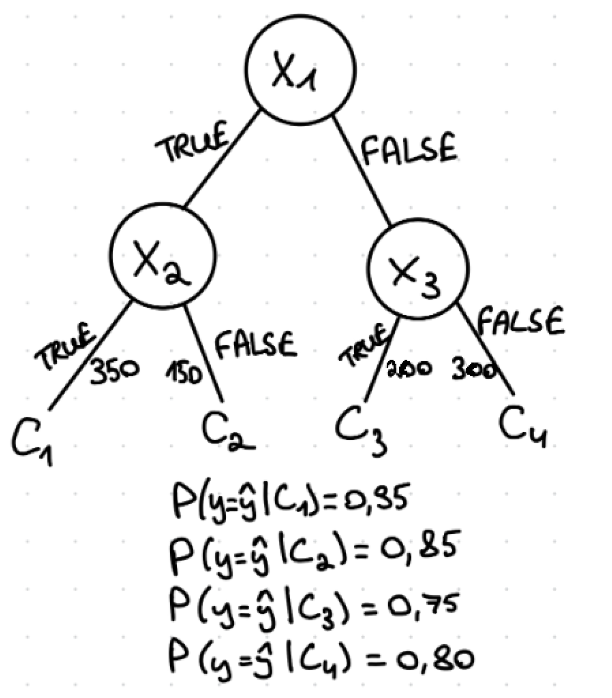
\includegraphics{Screenshot 2025-01-09 at 11.52.49.png}
\subsubsection*{Explanation of Information Gain Calculation}

\paragraph{1. Parent Node Entropy \(H(D)\):}
The dataset contains \(1000\) examples in total:
\begin{itemize}
    \item Correctly classified: \(740\),
    \item Incorrectly classified: \(260\).
\end{itemize}

The probabilities are:
\[
P(\text{Correct}) = \frac{740}{1000} = 0.74, \quad P(\text{Incorrect}) = \frac{260}{1000} = 0.26.
\]

The entropy of the parent node is:
\[
H(D) = - \left( 0.74 \log_2(0.74) + 0.26 \log_2(0.26) \right)
\]
\[
H(D) \approx - \left( 0.74 \cdot (-0.432) + 0.26 \cdot (-1.943) \right) \approx 1.247.
\]

\paragraph{2. Weighted Child Node Entropies:}
After splitting on \(X_1\), we calculate the weighted entropy of the child nodes.

\subparagraph{a. For \(C_1 + C_2\) (TRUE branch):}
\begin{itemize}
    \item Total examples: \(500\),
    \item Correct: \(350\),
    \item Incorrect: \(150\).
\end{itemize}

The probabilities are:
\[
P(\text{Correct}) = \frac{350}{500} = 0.7, \quad P(\text{Incorrect}) = \frac{150}{500} = 0.3.
\]

The entropy is:
\[
H(C_1, C_2) = - \left( 0.7 \log_2(0.7) + 0.3 \log_2(0.3) \right)
\]
\[
H(C_1, C_2) \approx 0.881.
\]

\subparagraph{b. For \(C_3 + C_4\) (FALSE branch):}
\begin{itemize}
    \item Total examples: \(500\),
    \item Correct: \(390\),
    \item Incorrect: \(110\).
\end{itemize}

The probabilities are:
\[
P(\text{Correct}) = \frac{390}{500} = 0.78, \quad P(\text{Incorrect}) = \frac{110}{500} = 0.22.
\]

The entropy is:
\[
H(C_3, C_4) = - \left( 0.78 \log_2(0.78) + 0.22 \log_2(0.22) \right)
\]
\[
H(C_3, C_4) \approx 0.811.
\]

\subparagraph{c. Weighted Entropy After Split:}
\[
H_{\text{split}} = \frac{500}{1000} H(C_1, C_2) + \frac{500}{1000} H(C_3, C_4)
\]
\[
H_{\text{split}} = 0.5 \cdot 0.881 + 0.5 \cdot 0.811
\]
\[
H_{\text{split}} \approx 0.846.
\]

\paragraph{3. Information Gain:}
The information gain of the top-level node is:
\[
IG(D, X_1) = H(D) - H_{\text{split}}
\]
\[
IG(D, X_1) = 1.247 - 0.846 \approx 0.401.
\]

\subsubsection*{Conclusion}
The information gain for splitting on the top-level node \(X_1\) is approximately:
\[
IG(D, X_1) \approx 0.401.
\]

\newpage
\section*{Chapter 4: Neural Networks}
\begin{itemize}
	\item \textbf{Forward Propagation}: Compute activations layer by layer.
	\item \textbf{Backpropagation}: Update weights using gradients from the chain rule.
	\item \textbf{Activation Functions}:
	\begin{itemize}
		\item Sigmoid: \( \sigma(x) = \frac{1}{1 + e^{-x}} \).
		\item ReLU: \( \text{ReLU}(x) = \max(0, x) \).
		\item Tanh: \( \tanh(x) = \frac{e^x - e^{-x}}{e^x + e^{-x}} \).
	\end{itemize}
\end{itemize}
\section*{Chapter 5: Evaluating Hypotheses}
\section*{Chapter 6: Bayesian Learning}
\subsection*{Bayes' Theorem}
\[
P(H|E) = \frac{P(E|H)P(H)}{P(E)}
\]
where:
\[
P(E) = \sum_i P(E|H_i)P(H_i)
\]

\subsection*{MAP (Maximum A Posteriori)}
\[
H_{\text{MAP}} = \arg\max_H P(H|E) = \arg\max_H P(E|H)P(H)
\]

\subsection*{Naive Bayes Classifier}
\[
P(C|X) = \frac{P(C)\prod_{i=1}^{n}P(x_i|C)}{P(X)}
\]
\[
P(X|C) = \prod_{i=1}^{n}P(x_i|C)
\]

\subsection*{Bayesian Network Example (from WPO8)}
\[
P(a|c) = \frac{P(c|a)P(a)}{P(c)}
\]
where:
\[
P(c) = P(c|a)P(a) + P(c|\neg a)P(\neg a)
\]

\subsection*{Sum Rule}
\[
P(A) = P(A \cap B) + P(A \cap \neg B)
\]
\[
P(A \cup B) = P(A) + P(B) - P(A \cap B)
\]
\subsection*{Product Rule}
\[
P(A \cap B) = P(A|B)P(B)
\]

\subsection*{Theorem of Total Probability}
\[
P(E) = \sum_{i} P(E|H_i)P(H_i)
\]


\subsection*{Joint and Marginal Probabilities (from WPO8)}
\[
P(a, d|\neg b) = P(d|a, \neg b)P(a|\neg b)
\]
\[
P(d) = P(d|a, b)P(a, b) + P(d|a, \neg b)P(a, \neg b) + P(d|\neg a, b)P(\neg a, b) + P(d|\neg a, \neg b)P(\neg a, \neg b)
\]

\section*{Chapter 7: Computational Learning Theory}
\subsection*{Version Space and Candidate Elimination}
\begin{itemize}
	\item General-to-Specific Ordering: Hypotheses are refined iteratively using training examples.
	\item Version Space:
	\[
	VS_{H,D} = \{ h \in H : h \text{ consistent with } D \}.
	\]
	\item Find-S Algorithm:
	\begin{enumerate}
		\item Initialize \( S \) to the most specific hypothesis.
		\item Generalize \( S \) only as needed to be consistent with positive examples.
	\end{enumerate}
\end{itemize}

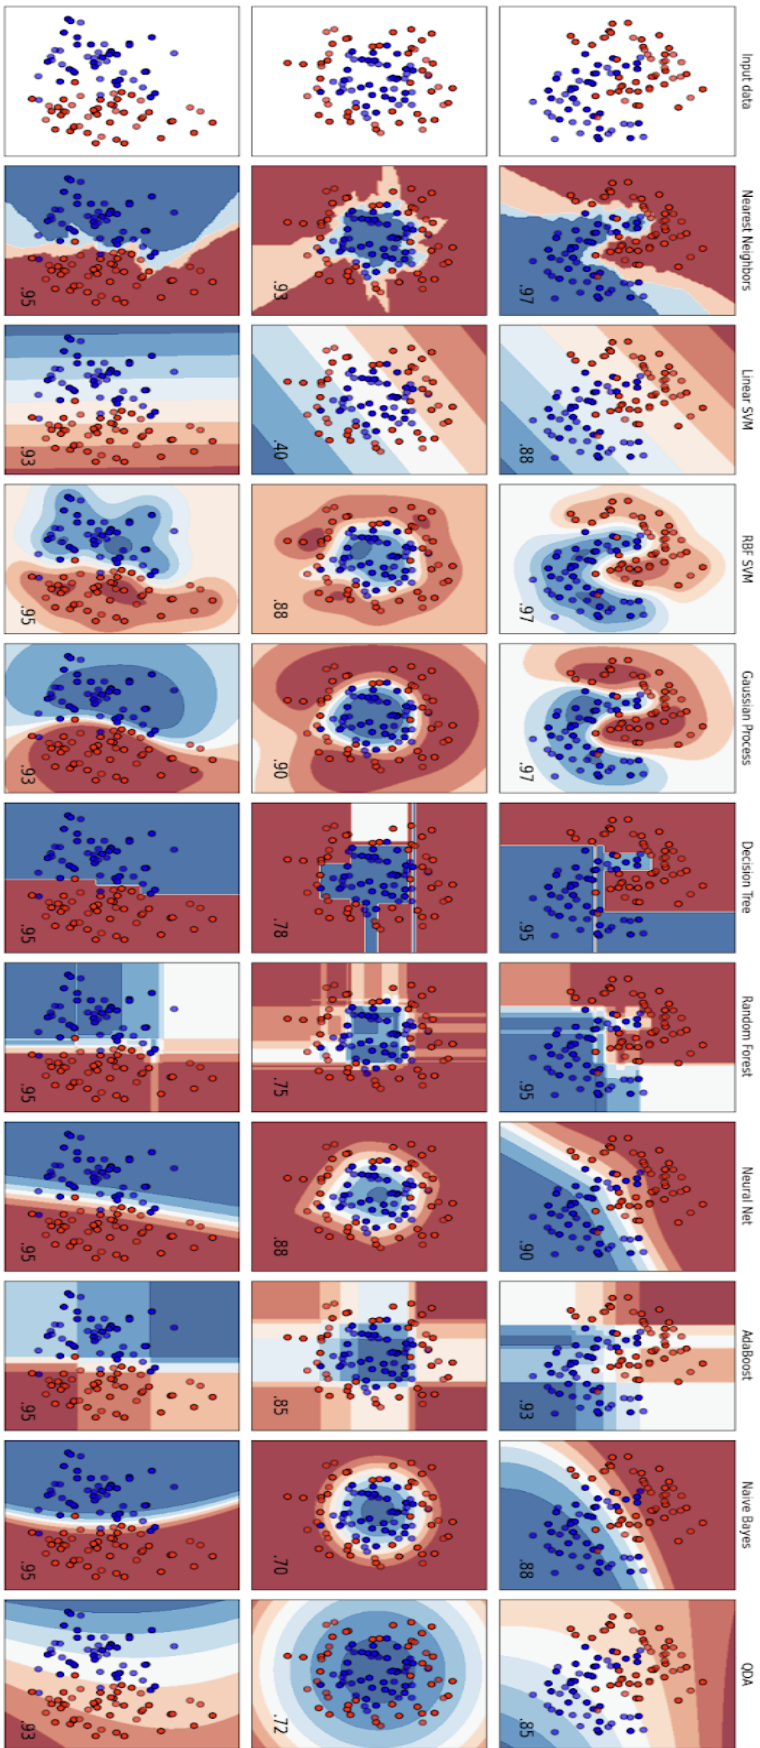
\includegraphics[scale=0.8]{Screenshot 2025-01-09 at 17.35.36.png}
\section*{Chapter 8: Instance-Based Learning}
\subsection*{k-Nearest Neighbors (k-NN)}
\begin{itemize}
	\item Lazy learner: Stores training data and computes distance during prediction.
	\item Distance Metric: Euclidean \( \sqrt{\sum (x_i - y_i)^2} \).
\end{itemize}


\section*{Chapter 10: Learning Sets of Rules}

\section*{Chapter 13: Reinforcement Learning}
\subsection*{Bellman Equation}
\[
V(s) = \max_a \left[ R(s, a) + \gamma \sum_{s'} P(s'|s, a)V(s') \right].
\]

\subsection*{Q-Learning Update Rule}
\[
Q(s, a) \leftarrow Q(s, a) + \alpha \left[ r + \gamma \max_{a'} Q(s', a') - Q(s, a) \right].
\]

\subsection*{Policy Iteration}
\begin{enumerate}
    \item Policy evaluation.
    \item Policy improvement.
\end{enumerate}


\section*{Machine Learning Questions and Answers}

\begin{itemize}
    \item \textbf{Increasing the depth of a decision tree cannot increase the training error: True.} Increasing the depth allows the tree to fit the training data perfectly, reducing the training error to zero.

    \item \textbf{It is generally a good idea to initiate the weight at 0 when doing gradient descent on the weights of a Neural Network: False.} Initializing weights to zero leads to symmetry breaking issues, making neurons in the same layer identical.

    \item \textbf{When two variables are independent, there is no correlation between them: True.} Independence implies no statistical relationship, leading to zero correlation.

    \item \textbf{A KNN model with N data samples and K dimensionality with $K >> N$ (using Euclidean distance) will perform well in general: False.} The curse of dimensionality makes distances less meaningful, degrading performance.

    \item \textbf{No algorithm exists for a linear regressor that can reach a local optimum by minimizing the mean squared error using gradient descent: False.} Linear regression with mean squared error has a convex loss function, ensuring convergence to the global optimum.

    \item \textbf{In Expectation Maximization, the choice of the initial step (E or M) does not matter for convergence: True.} The algorithm converges regardless of whether it starts with the E-step or the M-step.

    \item \textbf{It is always a bad idea to add noise to your training data: False.} Adding noise can regularize models and prevent overfitting, improving generalization.

    \item \textbf{In reinforcement learning $R(s, a, s') \leq Q^*(s, a)$ $\forall s, a, s'$: True.} $Q^*(s, a)$ accounts for immediate and future rewards, always being greater than or equal to the immediate reward.

    \item \textbf{A model that only uses a linear activation function always results in a linear regression model: True.} The composition of linear transformations results in a linear model.

    \item \textbf{If we have a dataset with N elements with K attributes and $K >> N$, then K-nearest neighbor is a good algorithm to classify this: False.} High dimensionality causes equidistance between points, reducing KNN's effectiveness.

    \item \textbf{Adding training examples in a dataset increases the variance: False.} More data reduces the model's dependence on specific instances, decreasing variance.

    \item \textbf{The quality of k-clustering is independent of the choices of the centroids: False.} Poor initial centroids can result in suboptimal clustering outcomes.

    \item \textbf{PAC bounds are guaranteed to be efficient if the data is chosen adversarially: False.} Adversarial data violates the assumptions of PAC learning, making the bounds inefficient.

    \item \textbf{A smaller hypothesis space means a higher chance of overfitting: False.} Overfitting typically occurs when the hypothesis space is too large and flexible.

    \item \textbf{The number of parameters in a Bayesian Network is exponential in the total number of arcs in the graph: False.} The number of parameters is exponential in the number of parents per node, not the total arcs.

    \item \textbf{Using an ensemble of models always leads to better performance compared to using a single model: False.} If individual models are weak or highly correlated, the ensemble may perform worse.

    \item \textbf{Q-learning always finds the optimal policy, if convergence is ensured: True.} Proper exploration and learning rate schedules guarantee convergence to the optimal policy.

    \item \textbf{In an MLP, if all neurons only use a linear activation function, the network can still model non-linear relationships in the data as long as it has enough layers: False.} A network with only linear activations is equivalent to a single linear model, regardless of depth.

    \item \textbf{In the k-means algorithm, the number of clusters (k) must be determined after the algorithm runs and the data points are assigned to clusters: False.} The algorithm requires $k$ as an input to initialize centroids and assign data points.

\end{itemize}

\end{document}

